\documentclass[10pt,letterpaper]{article}
\usepackage[margin=0.78in,headheight=17pt]{geometry}
\usepackage[T1]{fontenc}
\usepackage[utf8]{inputenc}
\usepackage{lmodern,microtype,parskip}
\usepackage{amsmath,amssymb}
\usepackage{xcolor,booktabs,longtable,tabularx,array,enumitem}
\usepackage[most]{tcolorbox}
\usepackage{fancyhdr,lastpage,titlesec,hyperref,listings}
\usepackage{tikz}
\usetikzlibrary{arrows.meta,positioning,shapes.geometric}
\definecolor{navy}{HTML}{17324D}
\definecolor{bluegray}{HTML}{43657D}
\definecolor{lightblue}{HTML}{EAF2F8}
\definecolor{linegray}{HTML}{CBD5DF}
\definecolor{softgray}{HTML}{F3F5F7}
\definecolor{accent}{HTML}{8E3B46}
\hypersetup{colorlinks=true,linkcolor=navy,urlcolor=bluegray,pdfborder={0 0 0}}
\urlstyle{same}
\titleformat{\section}{\Large\bfseries\color{navy}}{\thesection}{0.6em}{}
\titleformat{\subsection}{\large\bfseries\color{bluegray}}{\thesubsection}{0.5em}{}
\setlist[itemize]{leftmargin=*,itemsep=3pt,topsep=3pt}
\setlist[enumerate]{leftmargin=*,itemsep=3pt,topsep=3pt}
\setlength{\emergencystretch}{3em}
\renewcommand{\arraystretch}{1.22}
\setlength{\tabcolsep}{4pt}
\pagestyle{fancy}\fancyhf{}
\lhead{Secure Programming \& SAST Engineering}
\rhead{Engineering Documentation Suite}
\cfoot{\thepage\ / \pageref{LastPage}}
\newcolumntype{Y}{>{\raggedright\arraybackslash}X}
\newcommand{\checkbox}{\(\square\)}
\newcommand{\blankline}{\noindent\rule{\linewidth}{0.35pt}\par\vspace{4pt}}
\newcommand{\writearea}[1]{\par\begin{tcolorbox}[colback=white,colframe=linegray,boxrule=0.5pt,height=#1,sharp corners]\mbox{}\end{tcolorbox}\par}
\newtcolorbox{focusbox}[1]{colback=lightblue,colframe=bluegray,title=\textbf{#1},fonttitle=\bfseries,breakable}
\newtcolorbox{warnbox}[1]{colback=softgray,colframe=accent,title=\textbf{#1},fonttitle=\bfseries,breakable}
\lstset{basicstyle=\ttfamily\footnotesize,breaklines=true,frame=single,rulecolor=\color{linegray},backgroundcolor=\color{softgray},showstringspaces=false,columns=fullflexible,keepspaces=true,upquote=true}

\begin{document}
\begin{titlepage}
\vspace*{1.0in}
{\color{bluegray}\Large Engineering reference}\\[1.0em]
{\color{navy}\Huge\bfseries Secure Programming and SAST Engineering}\\[0.7em]
{\Large Architecture, analysis internals, review operations and standards crosswalk}\\[2.0em]
\rule{\linewidth}{1.0pt}
\vfill
\textbf{Source discipline:} Book-derived foundations are identified separately from current engineering extensions.\\
\textbf{Edition:} 29 October 2026
\end{titlepage}
\tableofcontents
\clearpage
\begin{focusbox}{Reading and provenance contract}
Foundation: Chess and West (2007), \emph{Secure Programming with Static Analysis}, 14 chapters. This handbook independently synthesizes its technical themes without reproducing extended passages. Current practice: NIST SSDF v1.1, CWE, OWASP SAMM, OASIS SARIF and current vendor documentation, as of October 2026. Specific product capabilities and legal obligations are version-dependent.
\end{focusbox}
\section{Operating Definition and Scope}
Static analysis assesses a program without executing the analyzed program. Static Application Security Testing (SAST) applies such analysis to security-relevant properties. Common methods include AST/pattern matching, type-state reasoning, control-flow analysis, dataflow/taint analysis, and semantic query engines. A scanner finding is an \emph{observation or hypothesis}; it is not a demonstration of exploitability or a certificate of absence. Complementary practices include security requirements, architecture risk review, manual code review, SCA, DAST, fuzzing, runtime instrumentation and penetration testing.
\subsection{Assurance claims}
Do not conflate scanner coverage with path completeness, CWE classification with risk, or warning counts with vulnerability prevalence. Scope and configuration, rule quality, compiler/model accuracy, included files, generated code and library summaries all influence evidence quality. For each claim store the commit, source set, tool/ruleset version, run identity, output hash and reviewer action.
\section{Anatomy of an Analyzer}
\begin{center}
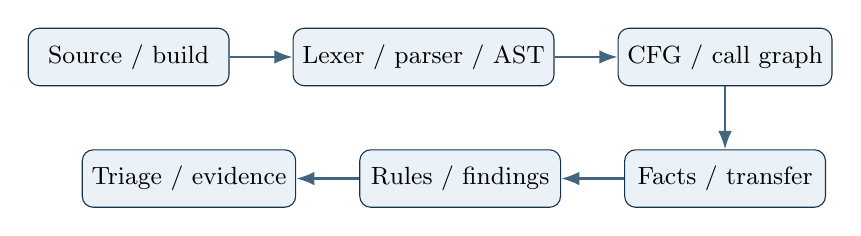
\begin{tikzpicture}[node distance=8mm, box/.style={draw=navy,fill=lightblue,rounded corners,align=center,minimum width=2.55cm,minimum height=0.73cm,font=\small},arr/.style={-Latex,thick,bluegray}]
\node[box](src){Source / build};\node[box,right=of src](ast){Lexer / parser / AST};\node[box,right=of ast](cfg){CFG / call graph};\node[box,below=of cfg](data){Facts / transfer};\node[box,left=of data](find){Rules / findings};\node[box,left=of find](triage){Triage / evidence};
\draw[arr](src)--(ast);\draw[arr](ast)--(cfg);\draw[arr](cfg)--(data);\draw[arr](data)--(find);\draw[arr](find)--(triage);
\end{tikzpicture}
\end{center}
\subsection{Analysis as a fixed-point computation}
A forward analysis computes \(OUT[n]=F_n(IN[n])\) and \(IN[n]=\bigsqcup_{p\in pred(n)} OUT[p]\). The state domain must be finite-height or use convergence mechanisms; monotonic transfer functions permit iterative fixed-point computation. A taint lattice may classify values as \(\{\mathrm{clean},\mathrm{tainted},\mathrm{unknown}\}\); real engines may track sources, paths, field sensitivities and validation semantics. The \emph{join} conservatively combines predecessor states. Interprocedural scope, call-string context, alias modeling and exception edges affect scalability and precision.
\subsection{Example property and query contract}
\begin{tabularx}{\linewidth}{@{}p{0.19\linewidth}Y@{}}\toprule
Element & Required specification\\\midrule
Source & Which API, input field or file is attacker-controlled, and under which trust assumptions?\\
Propagation & Through assignments, collections, aliases, return values or serializers\\
Sanitizer & Which operation actually neutralizes the particular sink syntax or enforces an invariant?\\
Sink & Security-critical API or operation with precondition (SQL execution, shell, path, HTML)\\
Finding & Path trace, rule identifier, location, confidence, CWE and review guidance\\\bottomrule
\end{tabularx}
\section{Precision, Soundness, Recall and Coverage}
A \emph{false positive} is an alert not representing the defined weakness in its actual application context; a \emph{false negative} is a missed occurrence. Confusion-matrix rates require a measured, representative labeled dataset. Without verified ground truth, do not report accuracy or false-positive rates from raw alert counts.
\[\mathrm{Precision}=\frac{TP}{TP+FP},\qquad \mathrm{Recall}=\frac{TP}{TP+FN}.\]
Report denominator, sampling method, adjudicator, deduplication rules, uncertainty and time window. Static analysis often trades soundness, path sensitivity, interprocedural context and compute budget. C/C++ build capture and macro expansion can change the effective source set; Java reflection and Python dynamic dispatch can limit models.
\section{Secure Coding Controls: Cross-Language Matrix}
\small
\begin{longtable}{@{}p{0.20\linewidth}p{0.24\linewidth}p{0.24\linewidth}p{0.24\linewidth}@{}}\toprule
Class & Java & C/C++ & Python\\\midrule\endhead
Injection & PreparedStatement; context-specific encoding & Avoid shell interpolation; explicit argv APIs & DB-API parameters; subprocess argument list with shell disabled\\
Memory safety & Bounds-checked collections; close resources & RAII, span/vector, checked sizes, sanitizers & Prefer typed APIs, avoid unsafe native extensions\\
Paths/files & Canonicalize, validate containment, use safe file APIs & openat-style designs and atomic flags; symlink threats & pathlib resolve plus containment; avoid race-sensitive check-then-open\\
Errors & try-with-resources; narrowed catch & RAII, error-code checks, exceptions per contract & with, explicit exceptions, structured safe logging\\
Secrets & Environment or managed secret service; avoid logs & Limit retention and copies; scrub where meaningful & Secret managers and minimized exception exposure\\
Authorization & Object and tenant check at service boundary & Least privilege and process sandboxing & Server-side authz before each data access\\\bottomrule
\end{longtable}
\normalsize
\section{Operational SAST Review Lifecycle}
\begin{enumerate}
\item \textbf{Authorize and scope}: repository, branch/commit, service, owner, sensitive data rules and permissible analyzers.
\item \textbf{Inventory and configure}: languages, build commands, rule packs, repository exclusions, dependency constraints and scan budgets.
\item \textbf{Establish baseline}: record existing findings with stable fingerprints, coverage gaps and an agreed historical backlog policy.
\item \textbf{Scan}: immutable revision, archived tool metadata, deterministic inputs as feasible, per-language categories, SARIF or native JSON.
\item \textbf{Triage}: validate the trace; classify weakness, exposure, reachability, privilege, impact, exploit prerequisites and data confidence.
\item \textbf{Remediate}: prefer root-cause or safe API changes over blanket suppressions; add negative and positive regression tests.
\item \textbf{Verify}: rerun affected tests and the scanner; confirm the finding is resolved, not merely excluded from detection.
\item \textbf{Govern}: record assigned ownership, authorized exceptions with expiry, change review, metrics and retest schedule.
\end{enumerate}
\subsection{Finding dispositions}
Use \emph{confirmed}, \emph{not a vulnerability / false positive}, \emph{needs investigation}, \emph{duplicate}, \emph{fixed verified}, and \emph{accepted risk (expiring)} as separate states. A false-positive claim needs code-path evidence; an accepted risk requires authority, treatment plan, expiration and compensating controls.
\section{Prioritization and Security Gates}
Use severity as one input, not an automatic decision. Record externally reachable entry points, privilege change, affected assets and confidentiality/integrity/availability impact. Gate candidate: block \emph{new, confirmed, high-impact} weaknesses under an agreed policy; fail open for scanner outage only through controlled break-glass with an audit trail. Existing baseline issues retain owners and SLAs; urgent exposure can override backlog sequencing. Never let an excluded path silently masquerade as passing coverage.
\subsection{Example measurable indicators}
\begin{tabularx}{\linewidth}{@{}p{0.29\linewidth}Y@{}}\toprule
Measure & Definition / guardrail\\\midrule
Scan execution rate & Successful required scans / eligible changes; report excluded and timed-out changes\\
Coverage proxy & Assessed in-scope modules / inventory modules; not a percentage of exploitable paths\\
Triage latency & Median time from introduction to first evidence-based disposition; report distribution\\
New confirmed findings & Unique confirmed issues introduced in the review window; exclude duplicates explicitly\\
Exception hygiene & Active approved exceptions with owner and future expiry / all active exceptions\\
Remediation verification & Fixes with scanner-plus-test verification / fixes submitted for closure\\\bottomrule
\end{tabularx}
\section{Threat Model for Scanner Infrastructure}
Scanner execution is a supply-chain boundary. An untrusted pull request may execute build scripts, package lifecycle hooks or analyzer extensions. Do not mix write privileges, secrets or deployment credentials into PR jobs. Use read-only token and isolated runners for untrusted source analysis; perform privileged SARIF upload in a separate, tightly scoped trusted context when permitted. Avoid privileged \texttt{pull\_request\_target} checkout of attacker-controlled code. Treat scanner config, query packs, caches, package downloads and output artifacts as potentially hostile inputs.
\section{SARIF, Deduplication and Evidence Lineage}
SARIF 2.1.0 records runs, tool identity, rules and results; location and stable fingerprint matter for alert tracking. Tool output is not necessarily compliant with every GitHub-specific SARIF subset. Validate schema, upload limits, result categories and permissions; distinguish raw scanner output from reviewed finding records. Avoid publishing private paths, stack traces and source snippets to untrusted artifact stores.
\section{SAST Boundaries and Adjacent Disciplines}
SAST is not a replacement for SCA (vulnerable dependencies), secret scanning (exposed credentials), IaC/container scanning, DAST, IAST, threat modeling or penetration testing. Some platforms combine engines in one product; report each control and its coverage independently. The textbook primarily covers code-level flaws; architecture and identity boundaries often require evidence beyond static analysis.
\section{Historical-to-Modern Crosswalk}
\begin{longtable}{@{}p{0.23\linewidth}p{0.32\linewidth}p{0.37\linewidth}@{}}\toprule
2007 book concept & Lasting principle & Modern translation or qualification\\\midrule\endhead
Fortify SCA + Audit Workbench labs & Scan, inspect, tune, audit, author rules & Versioned CI, CodeQL/Semgrep/maintained Fortify editions; commands and features vary\\
Java/C-centric examples & Language-specific trust and memory models & Java, C/C++, Python and cloud/service-specific flows\\
Review-cycle metrics & Feedback improves process & Differential findings, evidence-based false-positive sampling, baseline ownership\\
Seven Pernicious Kingdoms & Root cause taxonomy improves organization & CWE hierarchy, OWASP verification, risk-specific control mapping\\
Struts validation examples & Server-side authoritative input handling & Current web frameworks and API security requirements\\
Legacy runtime mitigation comparison & Defense-in-depth matters & Memory-safe language selection, sanitizers, hardened compilers, fuzzing\\\bottomrule
\end{longtable}
\section{Standards Register and Verification Dates}
\begin{itemize}
\item Chess, B. and West, J. (2007). \emph{Secure Programming with Static Analysis}. Addison-Wesley. Chapters 1--14, basis for foundational chapter structure.
\item NIST SP 800-218, SSDF v1.1 (final, February 2022), especially PW.7; \url{https://csrc.nist.gov/pubs/sp/800/218/final}. Rev.1 / SSDF v1.2 was an initial public draft as of the October 2026 source check, not treated as final here.
\item CWE, Common Weakness Enumeration and 2025 Top 25; \url{https://cwe.mitre.org/top25/}. Trends are prioritization aids, not vulnerability counts for a specific application.
\item OWASP SAMM Verification; \url{https://devguide.owasp.org/en/06-verification/}.
\item OASIS SARIF v2.1.0 and Errata 01; \url{https://www.oasis-open.org/standards/}.
\item GitHub, CodeQL action, SARIF uploads and secure workflow guidance; \url{https://github.com/github/codeql-action}, \url{https://docs.github.com/en/code-security}, \url{https://docs.github.com/en/actions/reference/security/secure-use}.
\item Semgrep product documentation; \url{https://semgrep.dev/docs/}. Verify command options, rule registry and licensing against the installed release.
\end{itemize}
\end{document}
